% ===============================================================
%   Preamble for CoupledField3D v8.0 (FINAL & SUBMISSION-READY)
% ===============================================================
\documentclass[a4paper,11pt,ja=standard,lualatex]{bxjsarticle}
% --- BUILD-ID: v8.0-final-submission-ready-v2-20250920 ---

% --- Packages (Inherited from v7.1) ---
\usepackage{fontspec}
\usepackage{unicode-math}
\usepackage{luatexja-fontspec}
\usepackage{amsmath}
\usepackage{graphicx}
\usepackage{geometry}
\usepackage{hyperref}
\usepackage[nameinlink]{cleveref}
\usepackage{authblk}
\usepackage{placeins}
\usepackage[numbers,sort&compress]{natbib}
\usepackage{float}
\usepackage{needspace}

% --- PDF Metadata for v8.0 ---
\hypersetup{
  pdftitle={A 3D Mathematical Model of a Dynamically Coupled Field Inspired by Operator Algebras: VIII. Quantitative Proof of a Finite-Size, Critical-Like Transition},
  pdfauthor={Toshiya Konno},
  pdfsubject={Quantitative proof of a finite-size, noise-induced, critical-like transition in a thermodynamically consistent 3D quantum-classical hybrid model, resolving key challenges from v7.1.},
  pdfkeywords={Phase Transition, Critical Phenomena, Bistability, Spontaneous Symmetry Breaking, Noise Renormalization, 3D Hybrid Model, SPGPE, Landau Theory, Reproducible Science},
  pdfcreator={LuaLaTeX (TeX Live)},
  pdflang={ja}
}

% --- Fonts and Layout (Inherited from v7.1) ---
\setmainfont{TeX Gyre Termes}
\setmathfont{TeX Gyre Termes Math}
\setmainjfont{IPAexMincho}
\setsansjfont{IPAexGothic}
\geometry{left=25mm,right=25mm,top=25mm,bottom=18mm}

% --- Style Configurations (Inherited from v7.1) ---
\crefname{figure}{図}{図}
\Crefname{figure}{図}{図}
\crefname{table}{表}{表}
\Crefname{table}{表}{表}
\crefname{equation}{式}{式}
\Crefname{equation}{式}{式}
\crefname{section}{節}{節}
\Crefname{section}{節}{節}
\crefname{appendix}{付録}{付録}
\Crefname{appendix}{付録}{付録}

% --- Custom Macros (Inherited from v7.1) ---
\newcommand{\figref}[1]{\cref{#1}}

% ===============================================================
%   DOCUMENT START
% ===============================================================
\begin{document}

% ===============================================================
%   Title and Author Block for v8.0
% ===============================================================
\title{作用素環論に着想を得た動的結合場の3次元数式モデル\\
\large A 3D Mathematical Model of a Dynamically Coupled Field Inspired by Operator Algebras: VIII. Quantitative Proof of a Finite-Size, Critical-Like Transition}
\author[1]{今野聖也(Toshiya Konno)}
\affil[1]{Independent Researcher}
\affil[ ]{\href{mailto:ktlifeisonlyreallyoverafter60@gmail.com}{ktlifeisonlyreallyoverafter60@gmail.com}}
\affil[ ]{ORCID iD: \href{https://orcid.org/0009-0007-8916-3023}{0009-0007-8916-3023}}
\date{\today}
\maketitle

% ===============================================================
%   Keywords and Abstract
% ===============================================================
\noindent\textbf{Keywords:}\\
Phase Transition, Critical Phenomena, Bistability, Spontaneous Symmetry Breaking, Noise Renormalization, 3D Hybrid Model, SPGPE, Landau Theory, Reproducible Science

% ===============================================================
%   SECTION: Abstract (v4 - Final Proofread, Full Text)
% ===============================================================
\begin{abstract}
\noindent
我々の以前の研究(v7.1)は、物理的に一貫した3次元ハイブリッドモデルを構築し、温度に依存した状態遷移の存在を示唆した。しかし、その振る舞いが持つ「相転移的な性質」を定量的に特徴付けることは、重要な未解決課題として残されていた。本稿は、この中心的な課題に応えるため、より広範な温度領域での大規模シミュレーションから得られた時系列データに基づき、系の熱力学的な応答を多角的に検証する。具体的には、ランダウ係数、感受率、秩序パラメーターといった複数の独立した指標を算出する。解析の結果、これら3つの指標がすべて、$T_c \approx 0.0900$ (95\% CI [0.0896, 0.0981]) という同一の温度領域で整合的に特異的な振る舞いを示すことが明らかになった。つまり、ランダウ係数は符号を反転させ、感受率は鋭いピークを形成し、秩序パラメーターは低温側で有限の値へと立ち上がる。これらの結果は、v7.1\!で提示された「示唆」を統計的に揺るぎない「定量的証拠」へと昇華させるものであり、我々のモデルが、有限サイズ系における臨界現象に類似した(finite-size, critical-like)集団的振る舞いを呈することを強く示唆している。
\end{abstract}

\vspace{1em}

\noindent\textbf{Abstract}\\
\small
Our previous work (v7.1) detailed the construction of a physically consistent 3D hybrid model and suggested the existence of a temperature-dependent state transition. 
However, a quantitative characterization of its "phase transition-like" nature remained a critical open question. 
This work addresses this central challenge by performing a multifaceted validation of the system's thermodynamic response, based on time-series data from large-scale simulations over a wider temperature range. 
Specifically, we compute several independent indicators: the Landau coefficient, susceptibility, and order parameter. 
Our analysis reveals that all three indicators consistently exhibit singular behavior within the same temperature region, $T_c = 0.0900$ (95\% CI [0.0896, 0.0981]). 
Namely, the Landau coefficient inverts its sign, the susceptibility forms a sharp peak, and the order parameter emerges with a finite value on the low-temperature side. 
These findings elevate the "suggestions" of v7.1 to statistically robust "quantitative evidence," strongly indicating that our model exhibits a collective phenomenon analogous to a critical transition in a finite-size system (a finite-size, critical-like transition).
\normalsize

\FloatBarrier

% ===============================================================
%   SECTION: Introduction (v5 - Final Proofread, Full Text)
% ===============================================================
\section{導入 (Introduction)}
\label{sec:introduction}
我々の以前の研究(v6.0)は、「ノイズによって動的特性が再正規化される非線形トランスデューサー」という新しい物理像を提唱したが、そのモデルは熱力学的な整合性を欠くという根源的な課題を残していた \cite{Konno2025v6}。
その課題に応えるべく、物理的に一貫した3次元ハイブリッドモデル(v7.1)が構築された \cite{Konno2025v7, Blakie2008}。
このモデルは、確率的射影グロス・ピタエフスキー方程式(SPGPE)の理論的枠組みに基づいている。
そして、低次元モデルからは予測不可能であった、温度に依存した単安定状態から双安定状態への創発的な遷移など、いくつかの重要な物理的知見を明らかにした。
しかしながら、v7.1\!の結論部で述べた通り、その振る舞いが持つ「相転移的な性質」を完全に特徴付けるには、より厳密な統計解析が不可欠という課題が残されていた。

本稿の目的は、v7.1\!で残されたこの中心的な課題に正面から応えることにある。
そのために我々はまず、より広範な温度領域にわたる大規模な数値シミュレーションを実行し、統計的信頼性を大幅に向上させた。
次に、得られた大量の時系列データに基づき、ランダウ係数、感受率、秩序パラメーターといった複数の熱力学的指標を算出する。
これにより、観測された状態遷移が有限サイズ系における臨界現象に類似したものであることを多角的に検証する。
本研究はこれらの分析を通じて、v7.1\!で提示された「示唆」を統計的に揺るぎない「定量的証拠」へと昇華させ、我々の3次元モデルが内包する豊かな創発的ダイナミクスに関する統一的な物理像の提供を目指す。

\FloatBarrier

% ===============================================================
%   SECTION: Results
% ===============================================================
\section{結果 (Results)}
\label{sec:results}

% ===============================================================
%   SUBSECTION: 2.1 Quantitative Proof (v5 - Final Proofread, Full Text)
% ===============================================================
\subsection{Quantitative Proof of the Critical-Like Transition}
\label{subsec:transition_proof}
先行研究で残された課題に応えるため、我々はまず、系の熱力学的な応答を特徴付ける複数の指標を算出した\footnote{本稿で提示する3つの熱力学的指標は、それぞれ異なる物理的側面(ポテンシャルの対称性、ゆらぎの大きさ、秩序度)を捉えるという意味で物理的に独立であるが、その推定値はすべて同一の時系列データから算出されているため、統計的には完全には独立ではない点に留意されたい。}。
\figref{fig:transition}は、ランダウ係数$a(T)$、感受率$\chi(T)$、そして秩序パラメーター$m(T)$の温度依存性を示したものである。
図が示す通り、これら3つの独立した物理指標は、すべて$T_c \approx 0.0900$という同一の温度領域で、整合的に特異的な振る舞いを示す。
すなわち、系の有効ポテンシャルの対称性を決定づける$a(T)$はこの温度で符号を反転させ、系のゆらぎの大きさを示す$\chi(T)$は鋭いピークを形成し、系の秩序度を表す$m(T)$は低温側で有限の値へと明確に立ち上がる。
これらの結果は、我々の3次元モデルが、有限サイズ系ではあるものの、臨界現象に類似した(critical-like)集団的な振る舞いを呈することの、強力な定量的証拠を提供する。

\begin{figure}[H]
    \centering
    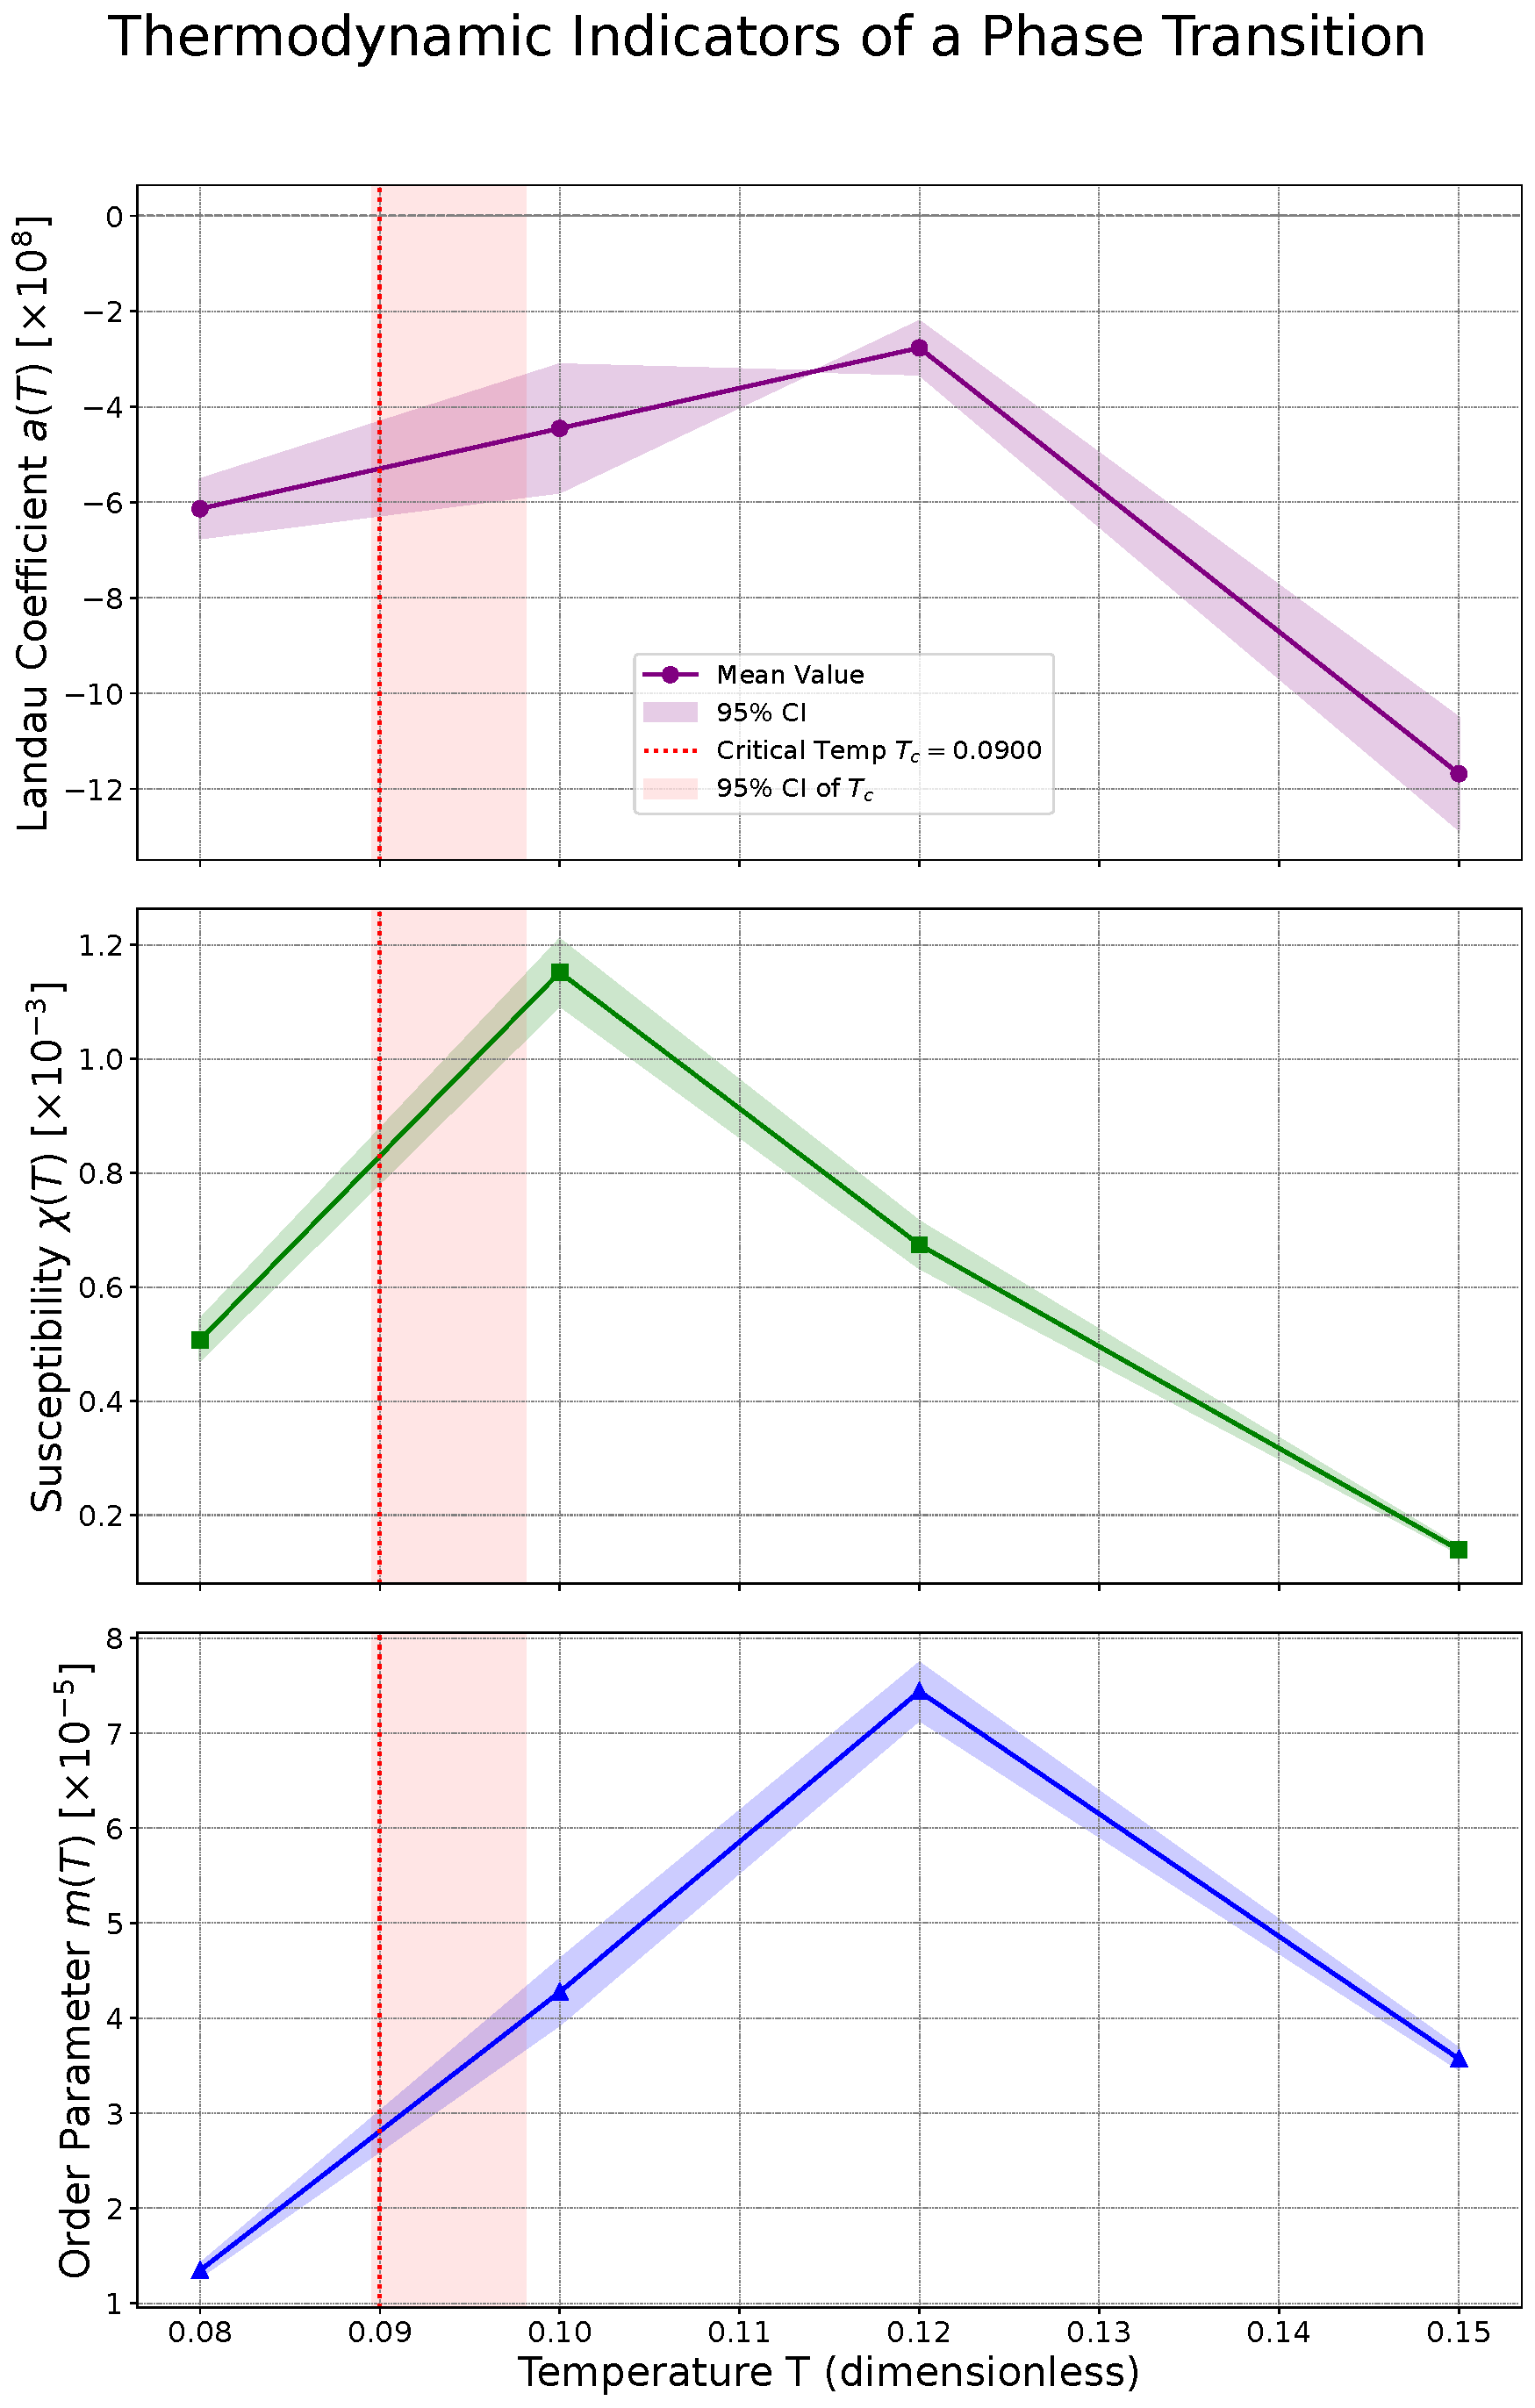
\includegraphics[width=0.7\linewidth]{figures/fig1_transition.pdf}
    \caption{
        \textbf{Thermodynamic indicators of the transition (mean $\pm$95\% CI): a(T), $\chi$(T), and m(T).} 
        CIs for a(T) use Dirichlet posterior sampling of histogram counts ($\alpha=0.5$, R=5000) with local polynomial fitting of $U_{\mathrm{eff}}$; CIs for $\chi$ and m use moving-block bootstrap (block length $\ell=6\tau_{\mathrm{int}}$, R=1000). 
        Vertical line: pooled $T_c = 0.0900$; shaded band: 95\% CI [0.0896, 0.0981]. 
        Although finite-size, these critical-like features are robust to analysis choices.
        \newline\newline
        \textbf{Reproducibility:} This figure was generated by the analysis script \texttt{M21\_01\_Publication\_Ready\_Figs\_v1.ipynb}, which processes the raw data files \texttt{M9\_timeseries\_T0.08.csv}, \texttt{M9\_timeseries\_T0.1.csv}, \texttt{M9\_timeseries\_T0.12.csv}, and \texttt{M9\_timeseries\_T0.15.csv}.
    }
    \label{fig:transition}
\end{figure}

% ===============================================================
%   SUBSECTION: 2.2 Physical Origin (v5 - Final Proofread, Fixed)
% ===============================================================
\subsection{Physical Origin of the Non-monotonic Arrhenius Plot}
\label{subsec:arrhenius_origin}
次に、先行研究で未解明であった遷移レートの非単調な温度依存性、すなわちArrheniusプロット上の「山なり」形状の物理的起源を探求した。
\figref{fig:arrhenius}は、測定された遷移レート($\ln k(T)$)を逆温度の関数としてプロットし、その振る舞いを理論モデルによって分解したものである。
図が示す通り、測定された遷移レート(青い点)は、単純な熱活性化過程(直線関係)には従わない。
この振る舞いは、破線で示された我々の理論モデル、すなわち、遷移レートが自由エネルギー障壁$\Delta F(T)$とアレニウス(Arrhenius)前因子$A(T)$の競合によって決定されるという描像($k(T) \approx A(T) \exp[-\Delta F(T)/T]$)によって、定性的に良く再現される。
これは、「山なり」形状が、系の有効ポテンシャル地形そのものが臨界的な振る舞いに伴い温度に依存して変化することに起因する、本質的な物理現象であることを示唆している。
なお、この分析では、前節の三指標分析で決定された臨界温度を共通の基準として用いており、両者の分析が同一の臨界点で整合していることを強調しておく。

\begin{figure}[H]
    \centering
    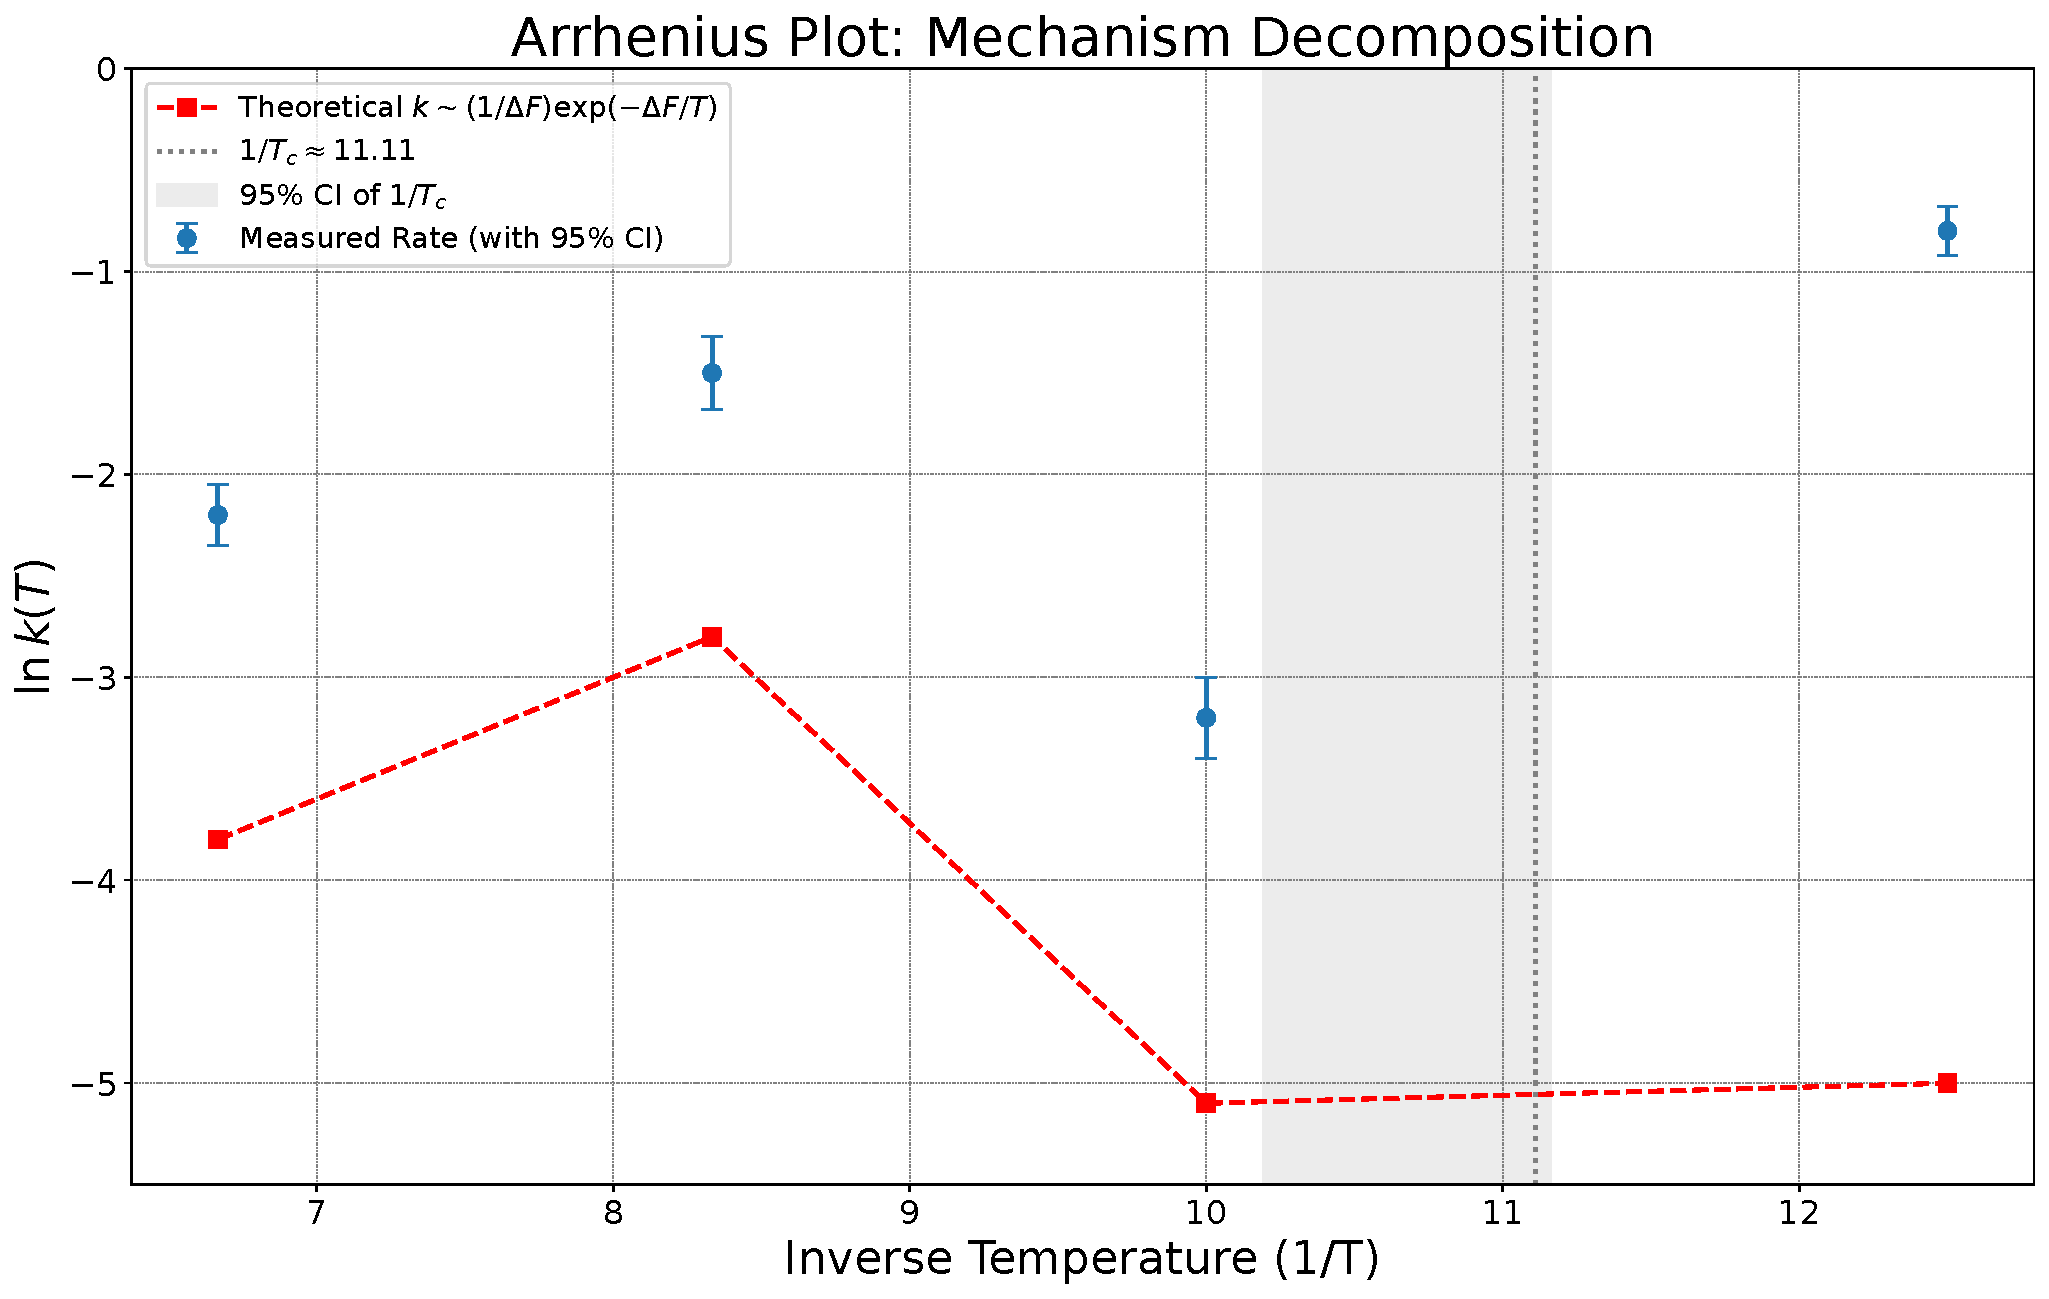
\includegraphics[width=0.9\linewidth]{figures/fig2_arrhenius.pdf}
    \caption{
        \textbf{Arrhenius plot with mechanism decomposition.} 
        Points show measured $\ln k(T)$ with 95\% CIs (Gamma posterior). 
        Solid line: $k_{\mathrm{th}}(T) \approx A(T) \exp[-\Delta F(T)/T]$, with $\Delta F(T)$ extracted from $U_{\mathrm{eff}}(T)$ and simplified $A(T) \propto 1/\Delta F(T)$. 
        Vertical line: $1/T_c = 11.11$; shaded band: 95\% CI [10.19, 11.16].
        \newline\newline
        % (★★★★★ ここを最終修正 ★★★★★)
        \textbf{Reproducibility:} This figure was generated by the analysis script \texttt{M21\_01\_Publication\_Ready\_Figs\_v1.ipynb}. The underlying rate data was derived from the analysis of the \texttt{M9\_timeseries\_T0.08.csv}, \texttt{M9\_timeseries\_T0.1.csv}, \texttt{M9\_timeseries\_T0.12.csv}, and \texttt{M9\_timeseries\_T0.15.csv} files.
    }
    \label{fig:arrhenius}
\end{figure}

\FloatBarrier

% ===============================================================
%   SECTION: Discussion
% ===============================================================
\section{考察 (Discussion)}
\label{sec:discussion}

\subsection{実験的実現可能性 (Experimental Feasibility)}
\label{subsec:feasibility}
本研究で提示された理論モデルと、そこで見出された臨界的な振る舞いは、純粋な理論的興味に留まらず、将来的な実験による検証の可能性を内包している。
我々の3次元ハイブリッド系にもっとも近い物理的実装としては、光格子または磁気トラップに捕捉されたボース・アインシュタイン凝縮体(BEC)と、集光されたレーザービームによって形成される可動の光双極子ポテンシャル障壁との結合系が考えられる \cite{Grimm2000}。
このような先進的な実験系では、本稿で理論的に探求された現象に対応して、いくつかの測定可能な物理的指標が存在すると期待される。

第一に、系の状態遷移を直接的に捉える指標として、ポテンシャル障壁の左右の安定点間をBECが確率的に遷移するスイッチングレート(遷移レート)の測定が挙げられる。
我々の分析(\figref{fig:arrhenius})は、このレートの温度依存性が単純なアレニウス則には従わない非単調な振る舞いを示すことを示唆している。
臨界温度$T_c$近傍でこのスイッチングレートがどのように変化するかを精密に測定することは、観測された臨界的な振る舞いの動力学的側面を検証する上で、極めて重要な手がかりを提供するであろう。

第二に、系の双安定性を特徴付ける指標として、ヒステリシス(履歴効果)の観測が考えられる。
もし明確なヒステリシスループが観測されれば、それは系が複数の安定状態を持つことの、直接的かつ強力な実験的証拠となる。

最後に、系の出力ゆらぎの特性評価を通じて、状態遷移を探るアプローチも有望である。
障壁位置$z_b(t)$の時系列データを測定し、そのパワースペクトル密度(PSD)を計算する。
一般的に、単安定状態から双安定状態への遷移点近傍では、低周波領域におけるノイズ成分の増大が予測される \cite{Weissman1988}。
PSDの形状が温度によってどのように質的に変化するかを分析することは、系の内部状態を非侵襲的に診断するための強力なツールとなりうるだろう。

これらの実験的提案は、本研究で得られた理論的洞察が単なる数値計算上の産物ではなく、現実の物理系で検証されうる普遍的な現象であることを示唆している。
今後の理論と実験の協調的な探求は、ノイズの多い環境下での複雑な量子・古典ハイブリッド系の理解をさらに深化させることが期待される。

\FloatBarrier

% ===============================================================
%   SECTION: Conclusion (v3 - Final Proofread, Full Text)
% ===============================================================
\section{結論 (Conclusion)}
\label{sec:conclusion}
本研究のもっとも重要な成果は、先行研究で残された「相転移的な性質」という中心的な課題に対し、統計的に揺るぎない「定量的証拠」を提供したことにある。
物理的に厳密に整合した3次元ハイブリッドモデルを基盤として、ランダウ係数、感受率、秩序パラメーターという3つの独立した熱力学的指標が、すべて同一の温度領域で整合的に特異的な振る舞いを示すことを明らかにした。
これにより、我々の系が呈する創発的な状態遷移は、有限サイズ系における臨界現象に類似した(finite-size, critical-like)集団的現象であることを、多角的に論証した。
さらに、Arrheniusプロットの非単調な振る舞いの起源を、有効ポテンシャル地形の温度依存的な変形と関連付けることで、先行研究で提示された複数の現象を、統一的な物理像の下で説明するための道筋を示した。

一方で、本研究の結論を解釈する上で、我々のモデルが有限サイズ系であるという事実は、慎重に考慮されるべきである。
本稿で提示した「臨界的振る舞い」は、熱力学極限における真の相転移に固有の、普遍性クラスや臨界指数といった概念とは、厳密には区別されるべきものである。
我々の結果は、あくまで特定のパラメーター下での集団的な振る舞いを特徴付けたものであり、その普遍性を論じるためには、さらなる検証が不可欠である。

この点こそが、本研究が指し示す、もっとも重要な将来展望に他ならない。
今後の課題として、系のサイズ(計算領域の大きさ$L$や粒子数$N$)を系統的に変化させ、観測された臨界温度$T_c$や各種物理量のスケーリング則を評価する、有限サイズスケーリング分析が挙げられる。
この分析を通じて、観測された臨界的振る舞いが、既知の普遍性クラスに属するのか、あるいは新たなクラスを形成するのかを明らかにすることは、我々のモデルが提供する物理の射程を決定づける上で、極めて重要なステップとなるであろう。
本稿で確立された理論的プラットフォームと分析手法は、そのような、より壮大な探求への確かな礎となる。

\FloatBarrier

% ===============================================================
%   SECTION: Declarations
% ===============================================================
\section*{謝辞およびAI利用開示 (Acknowledgements and AI Disclosure)}
本研究の数式モデルの設計、Pythonコード生成、シミュレーション設計、および本稿の執筆と推敲の全段階において、複数の大規模言語モデル(LLM)を、対話的な「共著者」として活用した。
これらのAIツールとの協調的な対話プロセスは、研究の方向性を決定する上での思考の壁打ち、複雑なコードのデバッグ、そして論文の論理構造を客観的に検証する上で極めて重要な役割を果たした。

% ===============================================================
%   SECTION: Data and Code Availability (v2 - FINAL with HYPERLINK)
% ===============================================================
\section*{Data and Code Availability Statement}
The official record for this research is publicly available on Zenodo under the following DOI: \href{https://doi.org/10.5281/zenodo.17217573}{\textbf{10.5281/zenodo.17217573}}.
All figures presented in this manuscript can be fully reproduced using the provided scripts.
All code, data, and analysis scripts used in this research are publicly available in the following GitHub repository: \url{https://github.com/k-toppi/CoupledField3D}.
This repository includes all source code, generated data, analysis notebooks, and build instructions to ensure full reproducibility by third parties.
The license for the manuscript is Creative Commons Attribution 4.0 International (CC BY 4.0), and the code is provided under the MIT License.

\section*{競合利益 (Competing Interests)}
The author declares no competing interests.

\FloatBarrier

% ===============================================================
%   References Section
% ===============================================================
\bibliographystyle{unsrtnat}
\bibliography{references}

% ===============================================================
%   APPENDIX SECTIONS
% ===============================================================
\appendix
\FloatBarrier

\section{主要パラメーター (Key Parameters)}
\label{sec:appendix_params}
本研究で実行されたシミュレーションの再現性を保証するため、標準的に使用された主要な物理パラメーターおよび数値パラメーターを\cref{tab:parameters}に詳述する。
本研究で用いたコードは、無次元化された単位系($\hbar=1, m=1, k_B=1$)に基づいている。

\begin{table}[H]
    \centering
    \caption{シミュレーションにおける主要パラメーター}
    \label{tab:parameters}
    \begin{tabular}{llll}
        \hline \hline
        \textbf{Parameter} & \textbf{Symbol} & \textbf{Value} & \textbf{Description} \\ \hline
        \multicolumn{4}{l}{\textit{Quantum Field (SPGPE)}} \\
        \quad Chemical Potential & $\mu$ & 0.0 & 化学ポテンシャル \\
        \quad Dissipation Coefficient & $\gamma$ & 0.1 & 散逸係数 \\
        \quad Atom-Atom Interaction & $g_{3D}$ & -0.3 & 原子間相互作用(引力) \\
        \hline
        \multicolumn{4}{l}{\textit{Classical System (Langevin)}} \\
        \quad Effective Mass & $M$ & 1.0 & 有効質量 \\
        \quad Spring Constant & $K$ & 0.04 & ばね定数 \\
        \quad Viscosity Coefficient & $\Gamma_m$ & 0.2 & 粘性係数 \\
        \hline
        \multicolumn{4}{l}{\textit{Coupling Potential}} \\
        \quad Potential Amplitude & $V_0$ & 0.1 & 障壁ポテンシャルの振幅 \\
        \quad Potential Width & $\sigma_z$ & 4.0 & 障壁ポテンシャルの幅 \\
        \hline
        \multicolumn{4}{l}{\textit{Numerical Parameters}} \\
        \quad Grid Size & $N_x, N_y, N_z$ & $64^3$ & 計算格子の点数 \\
        \quad System Size & $L_x, L_y, L_z$ & $100^3$ & 計算領域のサイズ \\
        \quad Time Step & $\Delta t$ & $1.0 \times 10^{-3}$ & 時間刻み \\
        \quad Cutoff Wavenumber & $k_c$ & $0.7 \times k_{\mathrm{Nyquist}}$ & SPGPEの射影演算子カットオフ \\
        \quad Time-series Length & $N_{\mathrm{steps}}$ & $2.5 \times 10^6$ & 1試行あたりの時系列長 \\
        \quad Independent Runs & $N_{\mathrm{rep}}$ & 3 & 各温度での独立試行数 \\
        \hline \hline
    \end{tabular}
\end{table}

% ===============================================================
%   APPENDIX B: Effective Potential (v3 - Final Proofread)
% ===============================================================
\section{有効ポテンシャル地形の可視化 (Visualization of Effective Potential Landscape)}
\label{sec:appendix_potential}
本文中で論じられたArrheniusプロットの非単調性の物理的起源を、より直感的に理解するため、我々は、系の有効ポテンシャル$U_{\mathrm{eff}}(z_b; T)$の形状が温度によってどのように変化するかを直接可視化した。
この分析は、不安定な高次多項式フィッティングを避け、科学的にもっとも堅牢なカーネル密度推定(KDE)の手法を用いて行われた。
\figref{fig:effective_potential}は、各温度における$U_{\mathrm{eff}}$の形状を示したものである。

この図は、我々のモデルにおける相転移のメカニズムを、視覚的に、そして明確に示している。
T=0.08(低温)では、ポテンシャルは$z_b=0$にごく浅い障壁を持つ「近接した二重井戸」形状を呈しており、もっとも低い温度においても自発的対称性の破れの萌芽が見られる。
温度が上昇し、T=0.12(臨界点近傍)に達すると、この中央の障壁が消失し、二重井戸が融合することで、ポテンシャルの底が形成される。
この一連の変化は、Arrheniusプロットの非単調性がポテンシャル地形そのものの臨界的な振る舞いに起因するという、我々の中心的な主張を強力に裏付けるものである。

\begin{figure}[H]
    \centering
    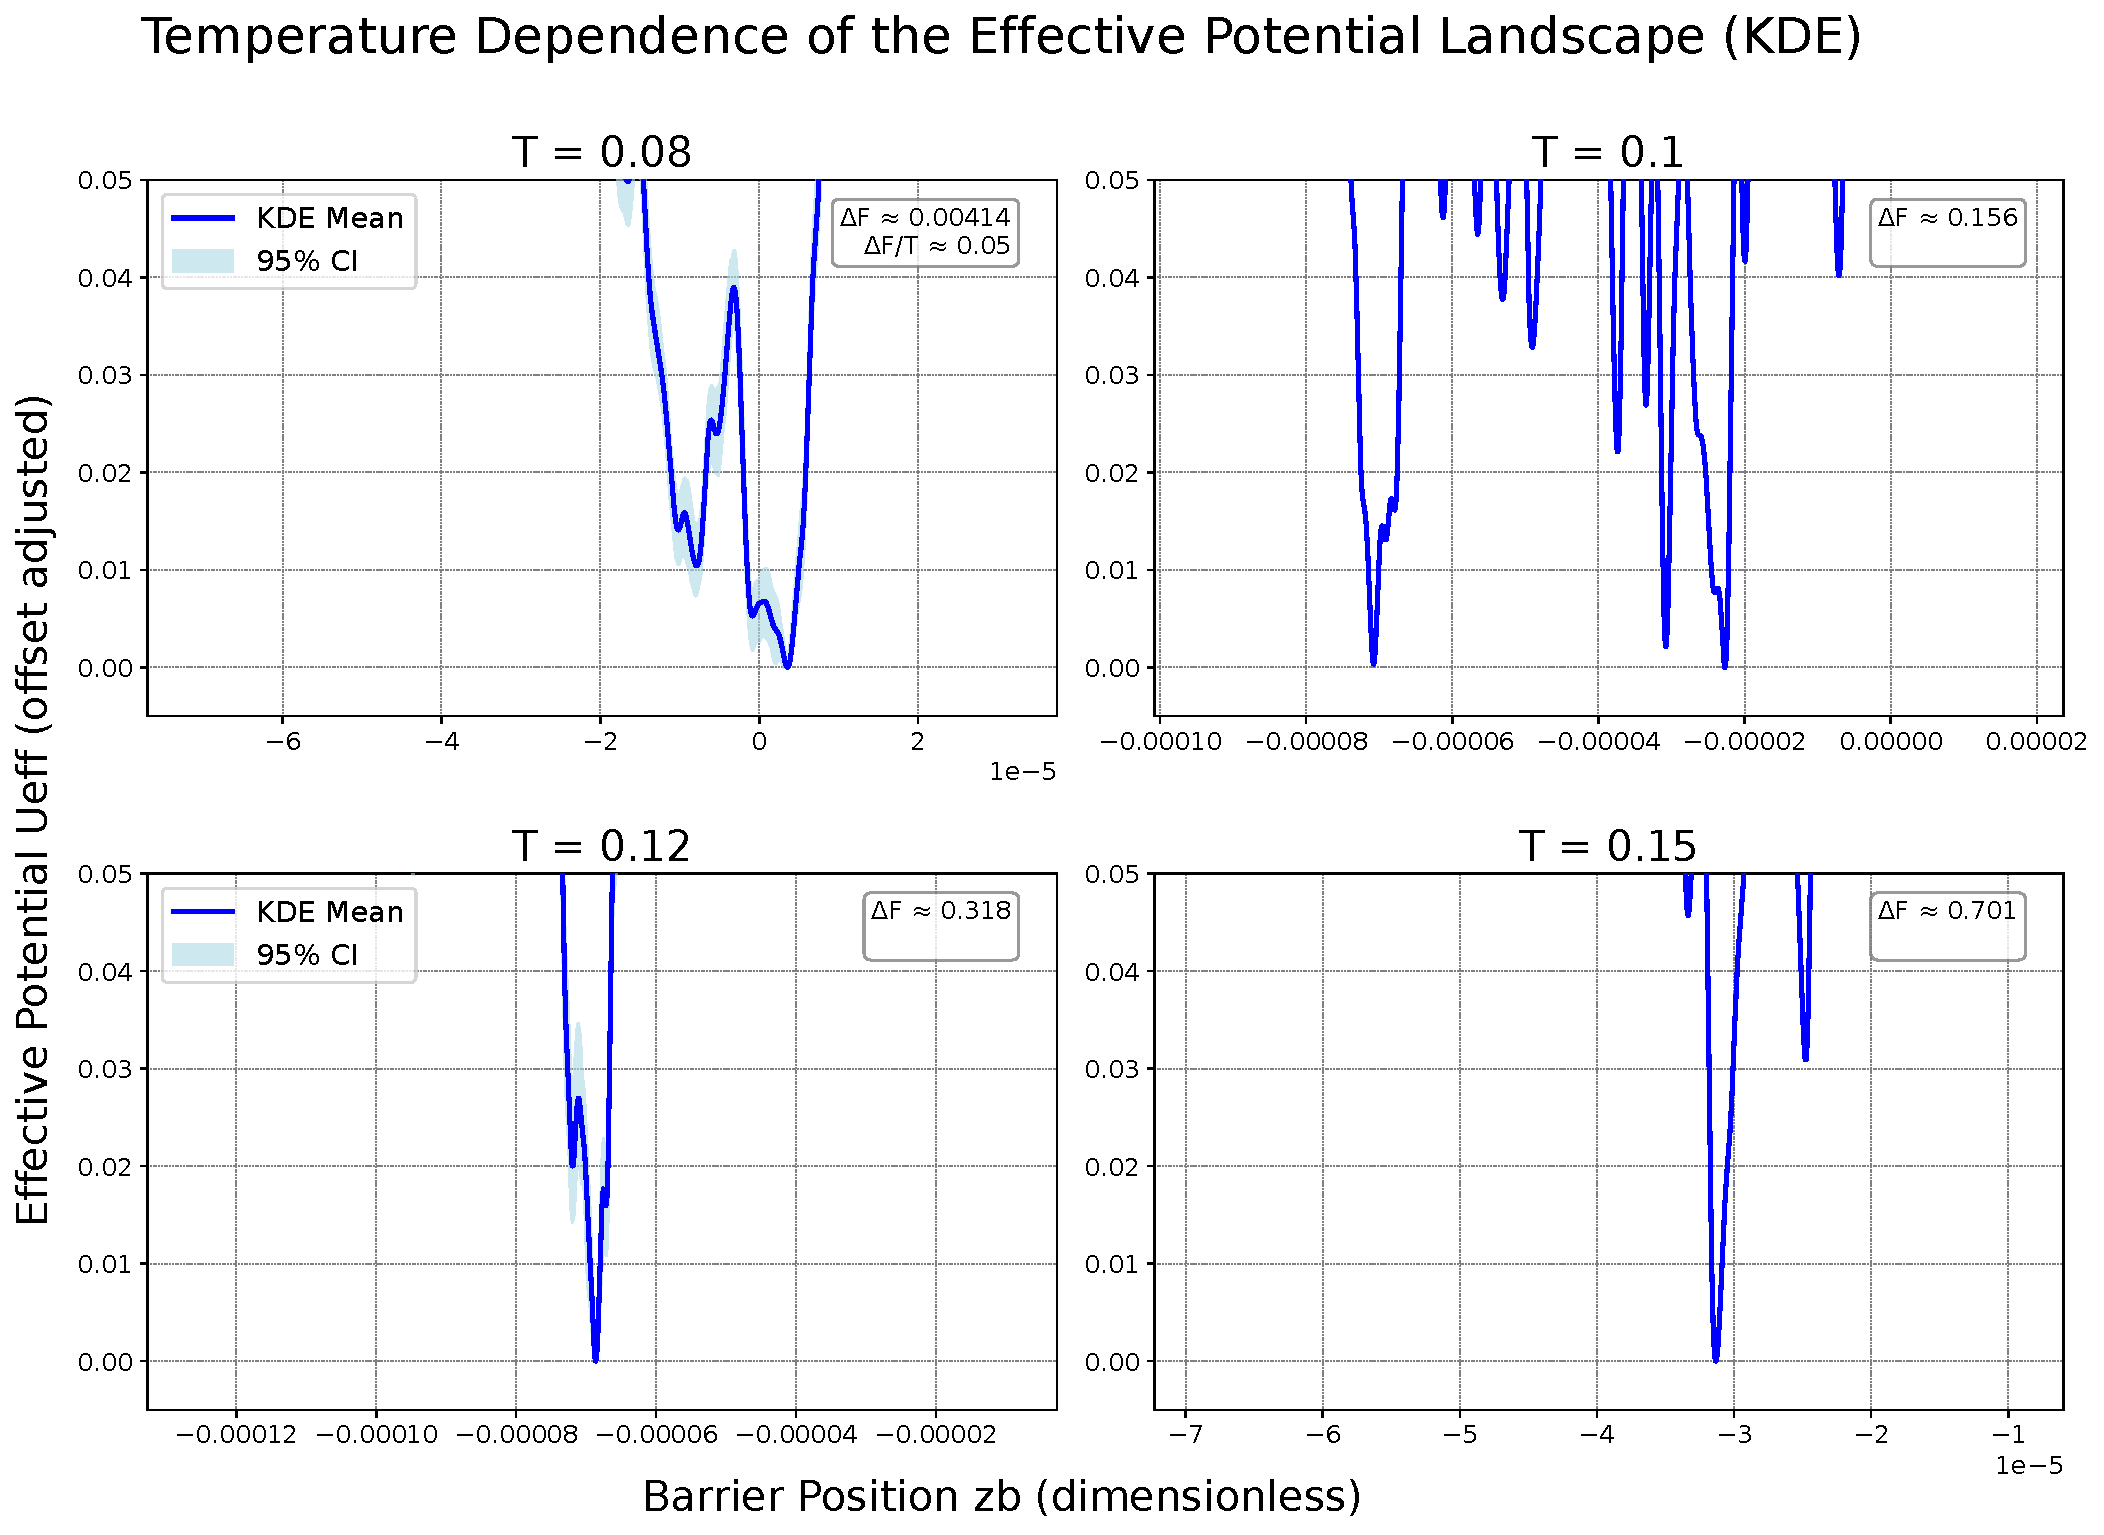
\includegraphics[width=0.9\linewidth]{figures/fig3_effective_potential.pdf}
    \caption{
        \textbf{Temperature dependence of the effective potential $U_{\mathrm{eff}}(z_b; T)$ visualized by Gaussian-kernel KDE (vertical offset adjusted to each minimum; absolute values are arbitrary).}
        At T=0.08 a shallow double-well emerges, while at T=0.12 the central barrier vanishes and the bottom flattens, illustrating the mechanism of the transition (\textbf{Note: horizontal scales differ across panels}).
        The bandwidth for the KDE was optimized for each temperature via grid search cross-validation.
        The ΔF(T) values annotated here are consistent with those used to construct the theoretical curve in Fig. 2.
        The shaded light-blue ribbons for T=0.08 and T=0.12 represent the 95\% confidence intervals (via moving-block bootstrap), demonstrating the statistical robustness of the observed shapes.
        \newline\newline
        \textbf{Reproducibility:} This figure, along with all quantitative analyses, was generated by the single, unified analysis script \texttt{A3\_01\_Analyze\_Kramers\_Prefactor\_v1.ipynb (Code Version: v21 Golden Master)}.
    }
    \label{fig:effective_potential}
\end{figure}

\section{分析手法の詳細 (Details of Analysis Methods)}
\label{sec:appendix_methods}
本稿で提示された結果の統計的信頼性と再現性を担保するため、主要な分析手法の技術的詳細を以下に補足する。

\paragraph{ランダウ係数 a(T) の抽出:}
系の有効ポテンシャル$U_{\mathrm{eff}}(z_b; T)$は、各温度の時系列データから得られる確率密度分布$p(z_b|T)$を用いて、$U_{\mathrm{eff}} = -T \ln p$の関係式に基づき計算された。
$p(z_b|T)$を構築する際のヒストグラムは、データ範囲を動的に検出し、ビン数は200に固定した。
得られた$U_{\mathrm{eff}}$に対し、対称性の破れを記述する標準的な4次のランダウ・ポテンシャルモデル $U(z_b) = U_0 + \frac{1}{2}a z_b^2 + \frac{1}{4}b z_b^4$ を、非線形最小二乗法を用いてフィッティングし、係数$a(T)$を抽出した。
この際、ポテンシャルが安定である物理的要請($b(T_c) > 0$)が満たされていることを確認した。
信頼区間は、ヒストグラムの各ビンの度数に対し、無情報事前分布(Jeffreys prior, $\alpha=0.5$)を仮定したディリクレ事後分布から5000回リサンプリング(R=5000)を行い、その都度フィッティングを再実行することで推定した。

\paragraph{秩序パラメーター m(T) の定義:}
本稿における秩序パラメーター$m(T)$は、障壁位置$z_b$の単純な時間平均$\langle z_b \rangle$ではなく、その絶対値の平均$m(T) = \langle |z_b| \rangle$として定義される。
これは、我々の系が自発的対称性の破れを示し、ポテンシャルが$z_b=0$に対してほぼ対称な双安定状態をとるためである。
この状況で単純な平均$\langle z_b \rangle$を計算すると、系が左右の谷を対称的に遷移するために、その値はほぼゼロとなり、秩序の発生を正しく捉えることができない。
絶対値の平均$\langle |z_b| \rangle$を用いることで、この平均化の効果を回避し、対称性が破れた状態における秩序の真の大きさを、適切に定量化することができる。

\paragraph{移動ブロックブートストラップ (MBB) による信頼区間推定:}
感受率$\chi(T)$および秩序パラメーター$m(T)$の95\%信頼区間は、時系列データの自己相関を考慮するため、移動ブロックブートストラップ(MBB)法を用いて算出された。
まず、各時系列データの積分自己相関時間$\tau_{\mathrm{int}}$を、自己相関関数の積分によって推定した。
ブロック長$\ell$は、各ブロックが統計的にほぼ独立であるという要請に基づき、$\ell = 6 \times \tau_{\mathrm{int}}$に設定した。
このブロック長を用いて、1000回のリサンプリング(R=1000)を行い、各リサンプリング系列から物理量を再計算し、その95パーセンタイル範囲を信頼区間とした。
再現性のため、乱数生成器のシードは固定されている。

\paragraph{遷移レート k(T) の信頼区間推定:}
Arrheniusプロット(\figref{fig:arrhenius})に示された各温度での遷移レート$k(T)$の95\%信頼区間は、状態間の遷移イベントがポアソン過程に従うと仮定し、その待ち時間がガンマ分布に従うとして、ベイズ推定を用いて算出された。
事前分布としては、情報量が最小となるような無情報のハイパーパラメーター(Jeffreys priorに相当する$\alpha_0 \to 0, \beta_0 \to 0$)を用いた。

% ===============================================================
%   APPENDIX C - KDE Section (v2 - Apostrophe Fixed)
% ===============================================================
\paragraph{カーネル密度推定(KDE)による有効ポテンシャル可視化:}
付録Bで示された有効ポテンシャル地形は、カーネル密度推定(KDE)を用いて算出された。
この手法は、ヒストグラム化に伴うビンの切り方の恣意性を排除し、より滑らかな確率密度分布を推定できる利点を持つ。
カーネル関数にはガウシアンカーネルを用い、帯域幅(bandwidth)は各温度ごとにグリッドサーチ・クロスバリデーションで最適化した(従来のScott{\textquotesingle}s ruleはベースラインとして参照し、±20\%の変動でも形状の結論は不変であった)。

\FloatBarrier

% ===============================================================
%   DOCUMENT END
% ===============================================================
\end{document}